\documentclass[20pt, a1paper, portrait]{tikzposter}
\usepackage[utf8]{inputenc}
\usepackage{graphicx}
\usepackage{amsmath}
\graphicspath{{./poster\_images/}}
\usepackage{xcolor}

\definecolor{eurecomblue}{RGB}{0,159,227}
\definecolor{visuwalkorange}{RGB}{255,204,0}



% RAJOUTER TITRE DU PROJET, AUTEURS
% 30% TEXTE, 40% ILLU, 30% VIDE
% PRECISER CHALLENGE TECHNIQUES
% RESULTATS
% CONCLUSION
% AMELIORATIONS, REFERENCES



\definebackgroundstyle{eurecom}{
\node[inner sep=0pt] at (0,0){
    
\includegraphics[width = \paperwidth,
    height = \paperheight]
    {poster-template.pdf}};
}

\defineblockstyle{bestblockstyle}{
titlewidthscale=0.9, bodywidthscale=1,titleleft,
titleoffsetx=0pt, titleoffsety=0pt, bodyoffsetx=0mm,
bodyverticalshift=10mm, roundedcorners=5,
titleinnersep=5mm, bodyinnersep=4mm,
bodyoffsety=8mm
}
{
\draw[color=eurecomblue, fill=blockbodybgcolor, line width=3pt,
rounded corners=\blockroundedcorners] (blockbody.south west)
rectangle (blockbody.north east);
\ifBlockHasTitle
\draw[color=eurecomblue, fill=eurecomblue
, line width=2pt,  
rounded corners=\blockroundedcorners] (blocktitle.south west)
rectangle (blocktitle.north east);
\fi
}

\usetitlestyle{Empty}

\usebackgroundstyle{eurecom}

\title {Visuwalk}

\titlegraphic{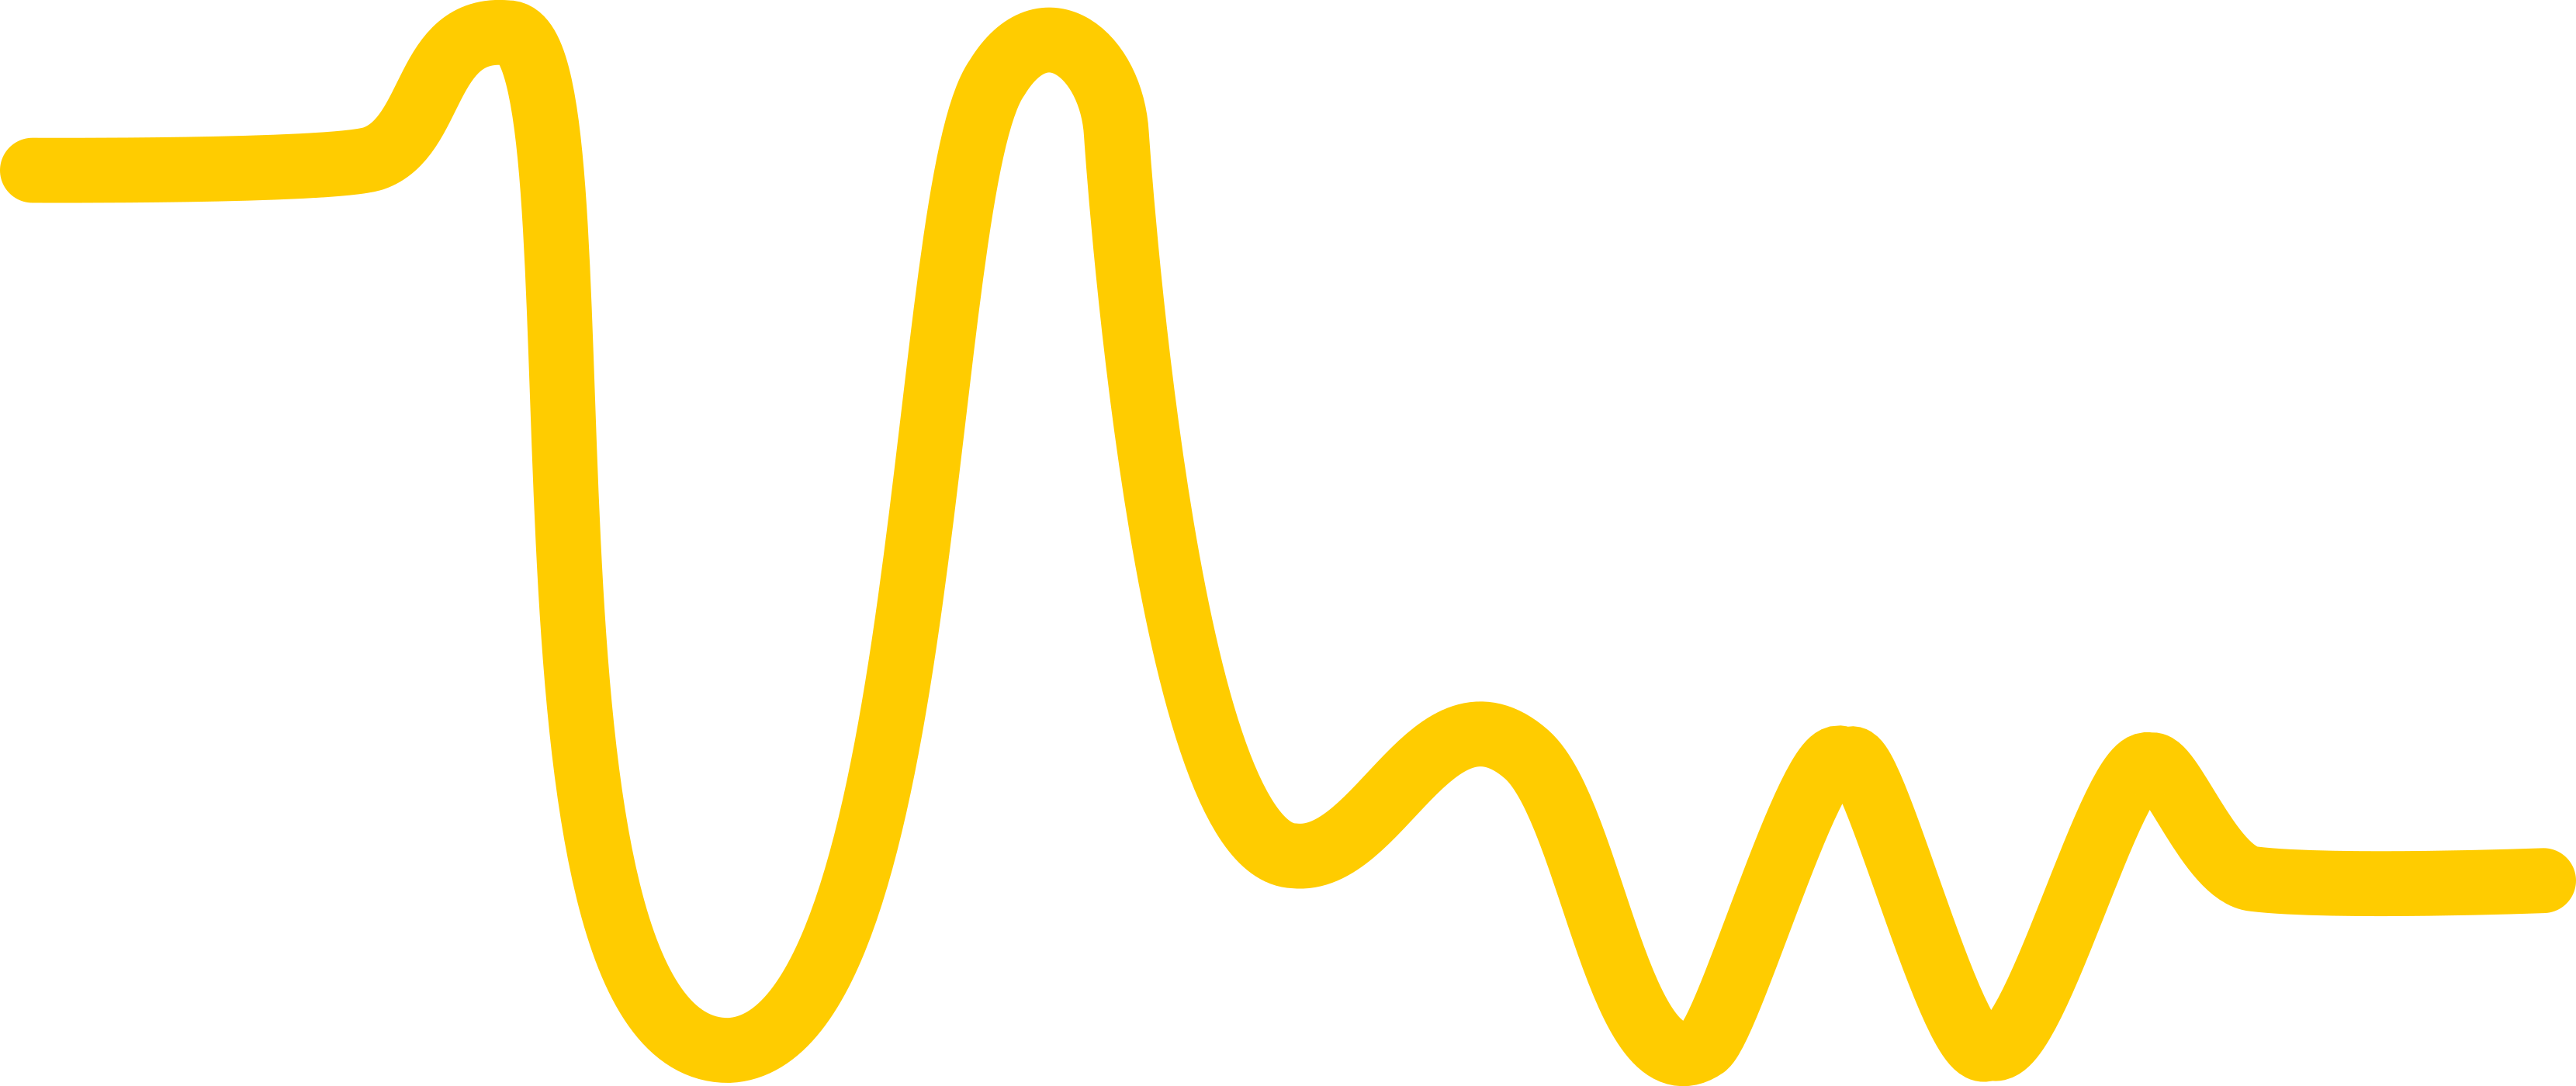
\includegraphics[width=0.20\paperwidth]{logo1.png}}
\author{\large Alexandre Avy, Hichem Khettab, Lou Marze, Hamza Parnica, Guillaume Ung}
\date{Semester 5}

\begin{document}

\useblockstyle{bestblockstyle}

\maketitle[titletotopverticalspace=90mm,width = 0.5\paperwidth]


\block[titleoffsety=30mm,bodyoffsety=38mm,bodyverticalshift=10mm,titleinnersep=5mm,bodyinnersep=4mm]{\textbf {Abstract}}{
\Large
The goal of this semester project is to guide ,with sounds, a visually impaired person to follow a line. \\
The available tools are a Rasperry Pi and its camera.
For this goal, one needs to : \\
Detect the line from the camera's video \\
Process the line with the right technique \\
Communicate instructions to the user
}

\begin{columns}

\column{0.5}

\block{
\textbf{Video Processing}}{

\begin{center} \LARGE {Detecting the line}
\end{center}

\vspace{2mm}
Prior to detecting the line, we process the image to optimize the detection quality through: \\
- Bilateral filtering \\
- Canny edge detection \\
Then we apply Hough transform to detect straight lines in the edges image.

\vspace{2mm}

\centering
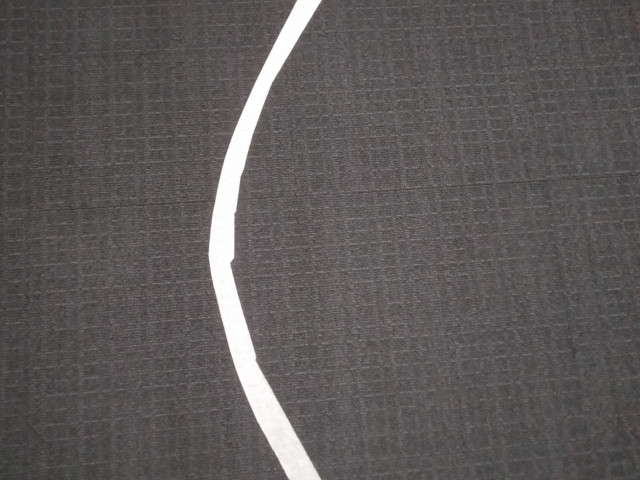
\includegraphics[height = 5cm, width = 5cm]{reel3.jpg}
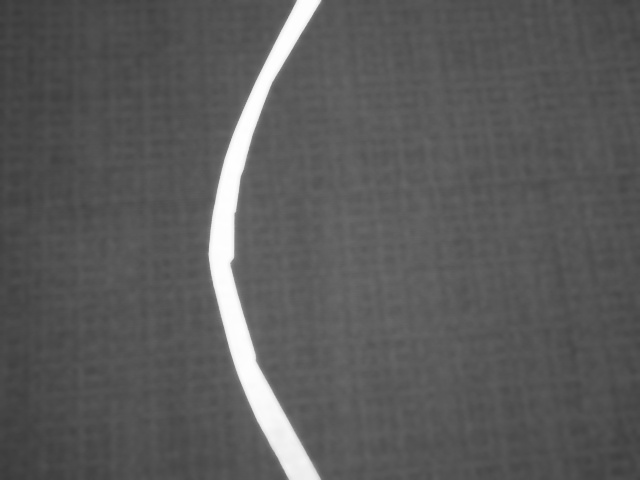
\includegraphics[height = 5cm, width = 5cm]{gray.jpg}
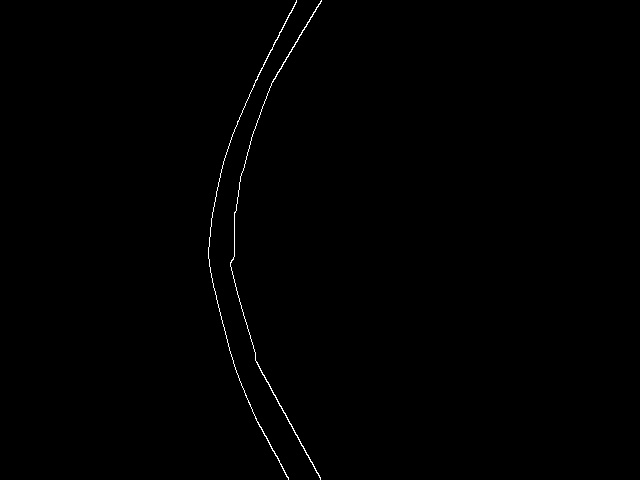
\includegraphics[height = 5cm, width = 5cm]{canny_edge.jpg}
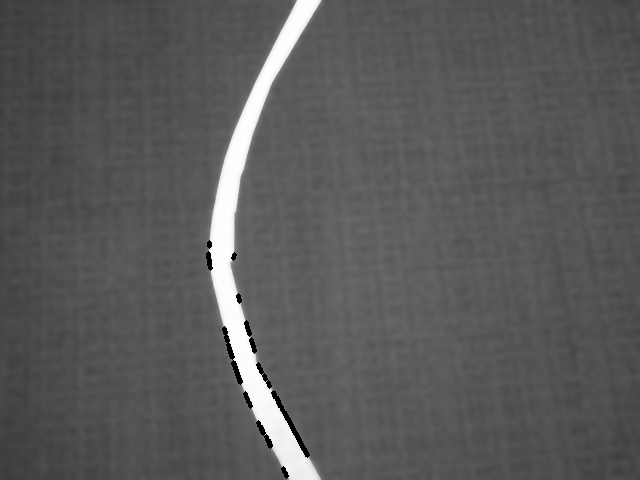
\includegraphics[height = 5cm, width = 5cm]{houghlines_maybe.jpg}
}



\column{0.5}

\block{
\textbf {Guiding the user}}{

}

\block{}{
We choose \(\tau\) so that \(d_{95\%} = \frac{w}{2}\), thus we have
\[ 3\tau = \frac{w}{2}, \quad \tau = \frac{w}{6} \]
It follows,
\[f(d) = 1 - e^{\frac{-6d}{w}}\]
}

\block{\textbf{Sound Processing}}{}

\end{columns}

\end{document}
